\makeatletter
\makeatother
\documentclass[../main.tex]{subfiles}

\graphicspath{
    {img}
	{../img/}
}

\begin{document}
\section{Корректная постановка задачи Коши}
\begin{definition}
Задача Коши для уравнения второго порядка с двумя независимыми переменными в области $D\in\R^2$ формулируется как:
\begin{equation} \label{eq:2.1.1}
    L(u) \equiv a_{11}\pderivTwo{u}{x}{x} + 2a_{12}\pderivTwo{u}{x}{y} + a_{22}\pderivTwo{u}{y}{y} + a\pderiv{u}{x} + b\pderiv{u}{y} + cu = f,
\end{equation}
\begin{equation} \label{eq:2.1.2}
    u\Bigr|_{(x, y)\in\textup{Г}} = \phi(x, y),\;\; \pderiv{u}{\Vec{n}}\Bigr|_{(x, y)\in\textup{Г}} = \psi(x, y),
\end{equation}
где $D$ - плоская область в $R^2$, Г - линия внутри области $D$, $u \in C^2(D)$, Г $\in C^2$, $\phi$ и $\psi$ - функции, заданные на линии Г.
\end{definition}
\begin{wrapfigure}{l}{0.55\textwidth}
          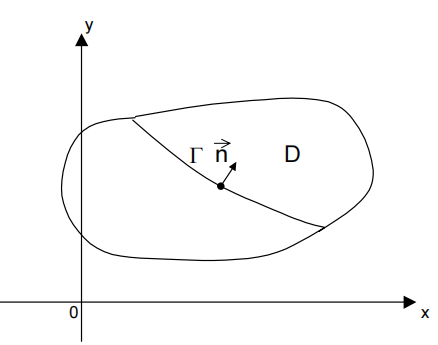
\includegraphics{2.1.PNG}
\end{wrapfigure}
Введём следующие пространства функций:
\begin{enumerate}
    \item $V_1$(Г) - пространство начальных функций $\phi$.
    \item $V_2$(Г) - пространство начальных функций $\psi$.
    \item $V$(D) - пространство  функций $u$, в котором отыскивается решение задачи (\ref{eq:2.1.1}), (\ref{eq:2.1.2}).
\end{enumerate}
Для классических решений: $V(D) \in C^2(D)$.\\
Будем предполагать, что пространства $V_1$, $V_2$, $V$ являются метрическими, то есть наделены расстояниями $\rho_1(\phi_1, \phi_2)$, $\rho_2(\psi_1, \psi_2)$, $\rho_3(u_1, u_2)$ между двумя функциями в соответственно $V_1$, $V_2$, $V$.\\
В случае нормированных линейных пространств:
\[
    \rho_1(\phi_1, \phi_2) = \|\phi_1 - \phi_2\|_{V_1},\;\;\;
    \rho_2(\psi_1, \psi_2) = \|\psi_1 - \psi_2\|_{V_2},\;\;\;
    \rho_3(u_1, u_2) = \|u_1 - u_2\|_V.
\]
\begin{definition}
Рассмотрим две задачи Коши с различными начальными функциями:
\begin{equation}
    L(u_i) = f,
\end{equation}
\begin{equation}
    u_i\Bigr|_{(x, y)\in\textup{Г}} = \phi_i,\;\;\;\pderiv{u_i}{\Vec{n}}\Bigr|_{(x, y)\in\textup{Г}} = \psi_i,\;\;\; i = 1, 2
\end{equation}
Решение задачи (\ref{eq:2.1.1}), (\ref{eq:2.1.2}) называется \textit{устойчивым по начальным данным}, если:
\begin{equation}
    \forall\mathcal{E}>0\;\exists\delta>0: \rho_1(\phi_1, \phi_2) < \delta,\; \rho_2(\psi_1, \psi_2) < \delta \implies \rho_3(u_1, u_2) < \mathcal{E}
\end{equation}
\end{definition}
\begin{definition}
Задача (\ref{eq:2.1.1}), (\ref{eq:2.1.2}) - \textit{корректно поставленная}, если $\forall\phi\in{V_1},\; \forall\psi\in{V_2}$:
\begin{enumerate}
    \item $\exists u\in{V}$.
    \item Решение $u$ единственно в $V$.
    \item Решение $u$ устойчиво по начальным данным.
\end{enumerate}
\end{definition}
\end{document}